In this section we outline the inputs that are used to discriminate between the 
SM Higgs signal and the dominant $W$ + jets background.  
The inputs are combined into a multivariate discriminant in order to maximize the 
separation.  
To describe the process at leading order, the maximal set of observables is given by~\cite{Gao:2010qx,Dobrescu:2009zf}:
\begin{equation}
\{ m_{l\nu jj}, m_{jj}, \cos\theta_1, \cos\theta_2, \Phi, \cos\theta^{\ast}, \Phi_1 \}
\end{equation}
The invariant mass of the leptonic $W$, $m_{l\nu}$, is constrained in the kinematic fit to compute the longitudinal momentum 
of the neutrino.  The angular variables are correlated and defined in Fig.~\ref{fig:anglesWWlvjj}.
%%%%%%%%%%%%%%%%%%%
\begin{figure}[ht]
  \centering
  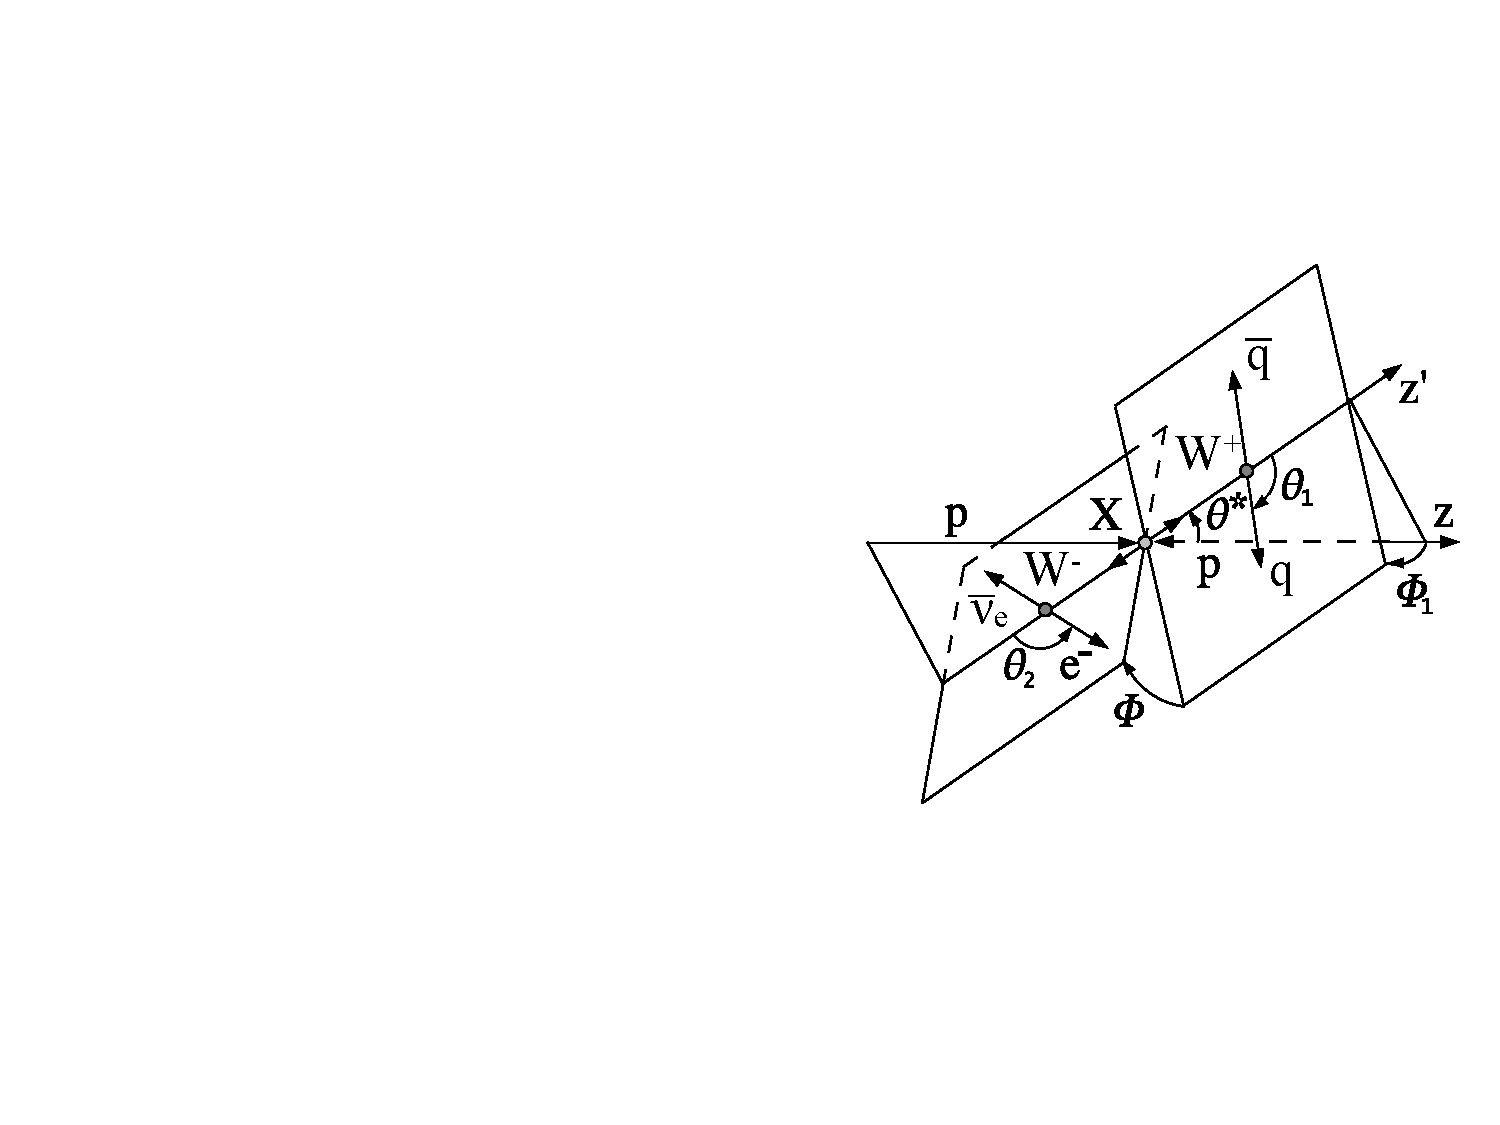
\includegraphics[width=0.5\textwidth]{figs/angles_wwlvjj.pdf}
  \caption{\label{fig:anglesWWlvjj}Angular definition for the $WW\to l\nu jj$ process}
\end{figure}
%%%%%%%%%%%%%%%%%%%
The angle $\cos\theta^{\ast}$ is the polar angle between the parton collision axis z and the $X$ 
decay axis $z'$, both defined in the $X$ rest frame. The angle $\Phi_1$ is the azimuthal angle
between the $zz'$ plane and the decay plane of hadronic $W$. The angles 
$\cos\theta^{\ast}$ and $\Phi_1$ are denoted as production
angles because they depend on the production mechanism, $gg$ or $q\bar{q}$.
For the SM Higgs which is a spin-zero particle, the production angles are flat (before acceptance). 
The angle $\Phi$ is the angle between the decay planes of the two $W$ systems in the $X$ rest
frame. The angle $\theta_i$ is the angle between
the direction of the fermion f from $W \to f\bar{f}$ and the direction opposite the $X$ in
the $W_i$ rest frame, where index i = 1, 2 refers to the first or second $W$ boson. 
In the case of the $\cos\theta_i$ angle from the hadronic $W$, it is ambiguous as to which jet is originating from the 
fermion or anti-fermion, so the angles is defined from $0$ to $\pi$ for the leading $p_T$ jet.  
Finally, The angles $\Phi$, $\cos\theta_1$ and $\cos\theta_2$ do not depend on the production mechanism and are denoted as the helicity angles.

The observables $m_{l\nu jj}$ and $m_{jj}$ are excluded from the MVA inputs.
The observable, $m_{l\nu jj}$, is not used because it is the distribution of this observable which is used
in the extraction of the upper limit.
The observable, $m_{jj}$, is not used since the $m_{jj}$ distribution is used to extract from the sideband to the signal region
to extract a data-driven shape for the background in the $m_{l\nu jj}$ spectrum. 
The leaves the five angular variables as inputs to the multivariate discriminant.  
As an example, the related search for the Higgs in the $ZZ \to 2l2q$ final state at CMS~\cite{CMS2l2q} uses these five observables
in an angular discriminant. 
Since the invariant masses are not used in the multivariate discriminant, the angular variables are defined in a loose window in 
$m_{l\nu jj}$ in order to take into account the correlations between the angles and the masses.  

In addition, to the five angular variables the $p_T$ of the WW system $p_{T,WW}$ 
and longitudinal boost (rapidity) $Y_{WW}$ are also used.  
The $Y_{WW}$ distribution comes from the parton distribution functions. 
The $p_{T,WW}$ distribution comes from next-to-leading order effects.  
The lepton charge is also included to give some discrimination power since the $W$ + jets background 
is asymmetric with respect to charge while the SM Higgs signal will be symmetric in lepton charge.  
These two quantities in addition to the mass and angular quantities form a full set of kinematic observables for process.
Other discriminating observables such as the $p_T$ of the $W\to jj$ system are not independent of the full set 
(and particularly of $m_{l\nu jj}$ and $m_{jj}$) are thus not used since they can sculpt the invariant mass distributions
to make the background more "signal-like".

%%Finally the quark-gluon likelihood discriminant observables for the two jets are used.  
%%The quark-gluon likelihood discriminant gives a measure of a jet originating from a quark or gluon~\cite{qgAN}
%%The SM Higgs signal consists of quark jets while the background is an admixture of both quark and gluon jets.  
%%
Combining all the inputs together the final set of inputs to the multivariate discriminant is:
\begin{equation}
\{ \cos\theta_1, \cos\theta_2, \Phi, \cos\theta^{\ast}, \Phi_1, p_{T,WW}, Y_{WW}, {\rm lepton~charge}\}
\end{equation}
%As an example, we plot the input variables for the SM Higgs mass of 300~GeV for the 2-jet $W\to\mu\nu$ category in Fig.~\ref{fig:inputs3002jmu}.


The distributions of input variables are shown in Figs~\ref{fig:inputs1702jmu}--\ref{fig:inputs6003jmu}
for various Higgs mass points and jet multiplicities.
%%%%%%%%%%%%%%%%%%%
\subsection{Input variables: \texorpdfstring{$M_H$}{M(H)} = 170~GeV, 2 jets}
%%%%%%%%%%%%%%%%%%%
\begin{figure}[ht]
  \centering
  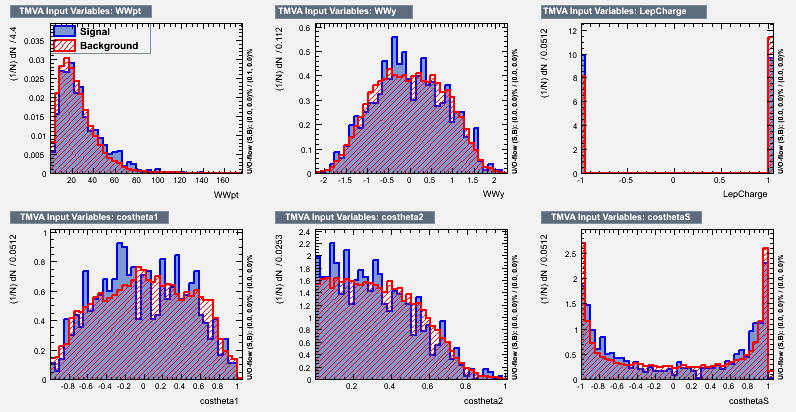
\includegraphics[width=0.8\textwidth]{figs/TMVA_170_nJ2_mu_variables_id_c1.png}
  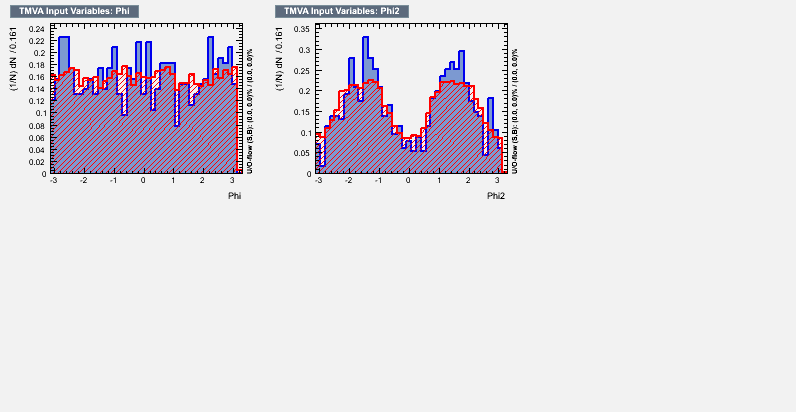
\includegraphics[width=0.8\textwidth]{figs/TMVA_170_nJ2_mu_variables_id_c2.png}	
  \caption{\label{fig:inputs1702jmu}Inputs to the multivariate discriminant for SM Higgs mass of 170~GeV for the 2-jet $W\to\mu\nu$ category}
\end{figure}
%%%%%%%%%%%%%%%%%%%
\newpage
\subsection{Input variables: \texorpdfstring{$M_H$}{M(H)} = 170~GeV, 3 jets}
%%%%%%%%%%%%%%%%%%%
\begin{figure}[ht]
  \centering
  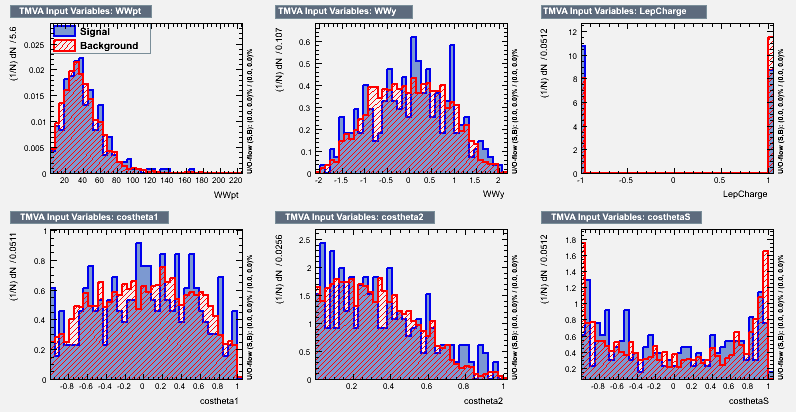
\includegraphics[width=0.8\textwidth]{figs/TMVA_170_nJ3_mu_variables_id_c1.png}
  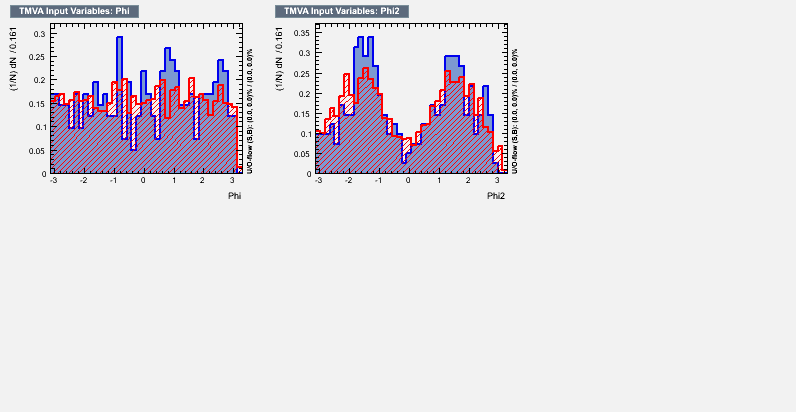
\includegraphics[width=0.8\textwidth]{figs/TMVA_170_nJ3_mu_variables_id_c2.png}	
  \caption{\label{fig:inputs1703jmu}Inputs to the multivariate discriminant for SM Higgs mass of 170~GeV for the 3-jet $W\to\mu\nu$ category}
\end{figure}
%%%%%%%%%%%%%%%%%%%
\newpage
\subsection{Input variables: \texorpdfstring{$M_H$}{M(H)} = 180~GeV, 2 jets}
%%%%%%%%%%%%%%%%%%%
\begin{figure}[ht]
  \centering
  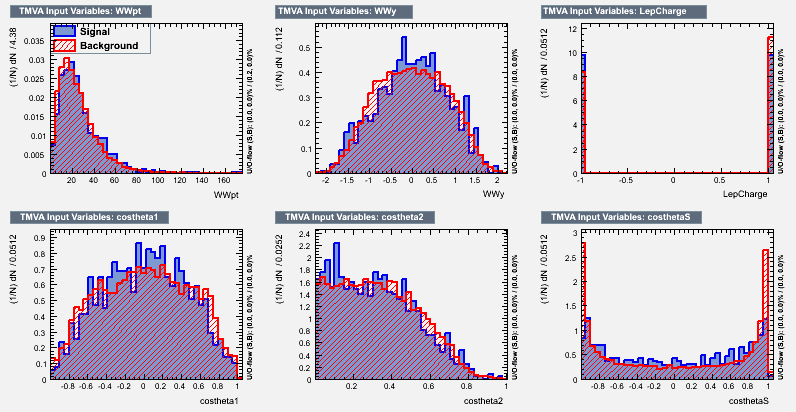
\includegraphics[width=0.8\textwidth]{figs/TMVA_180_nJ2_mu_variables_id_c1.png}
  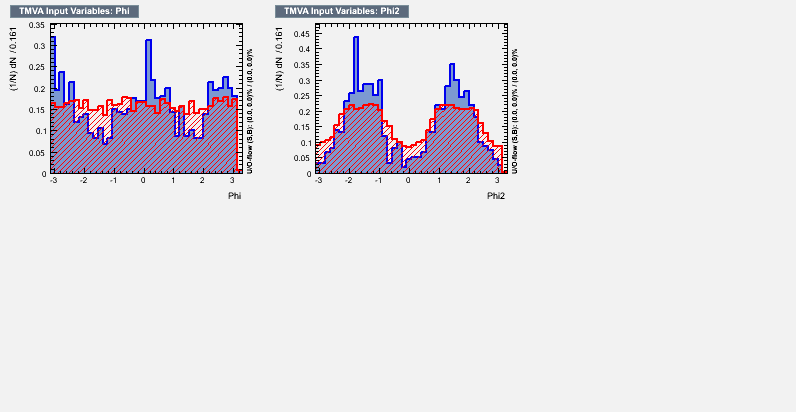
\includegraphics[width=0.8\textwidth]{figs/TMVA_180_nJ2_mu_variables_id_c2.png}	
  \caption{\label{fig:inputs1802jmu}Inputs to the multivariate discriminant for SM Higgs mass of 180~GeV for the 2-jet $W\to\mu\nu$ category}
\end{figure}
%%%%%%%%%%%%%%%%%%%
\newpage
\subsection{Input variables: \texorpdfstring{$M_H$}{M(H)} = 180~GeV, 3 jets}
%%%%%%%%%%%%%%%%%%%
\begin{figure}[ht]
  \centering
  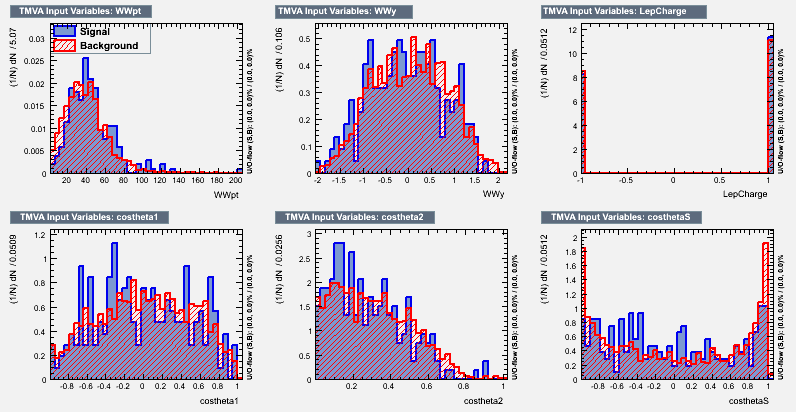
\includegraphics[width=0.8\textwidth]{figs/TMVA_180_nJ3_mu_variables_id_c1.png}
  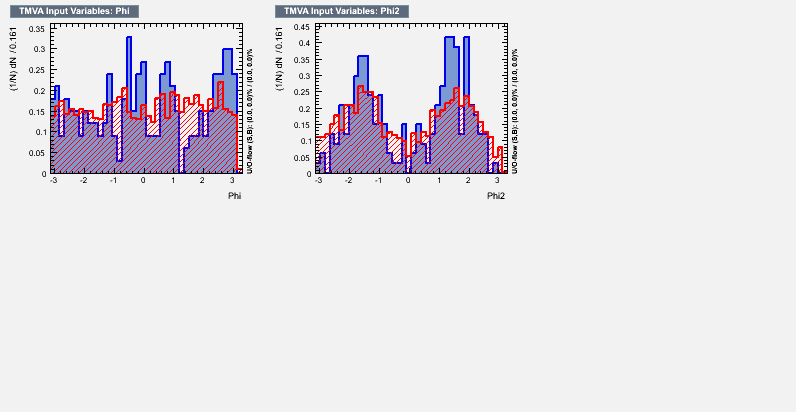
\includegraphics[width=0.8\textwidth]{figs/TMVA_180_nJ3_mu_variables_id_c2.png}	
  \caption{\label{fig:inputs1803jmu}Inputs to the multivariate discriminant for SM Higgs mass of 180~GeV for the 3-jet $W\to\mu\nu$ category}
\end{figure}
%%%%%%%%%%%%%%%%%%%
\newpage
\subsection{Input variables: \texorpdfstring{$M_H$}{M(H)} = 190~GeV, 2 jets}
%%%%%%%%%%%%%%%%%%%
\begin{figure}[ht]
  \centering
  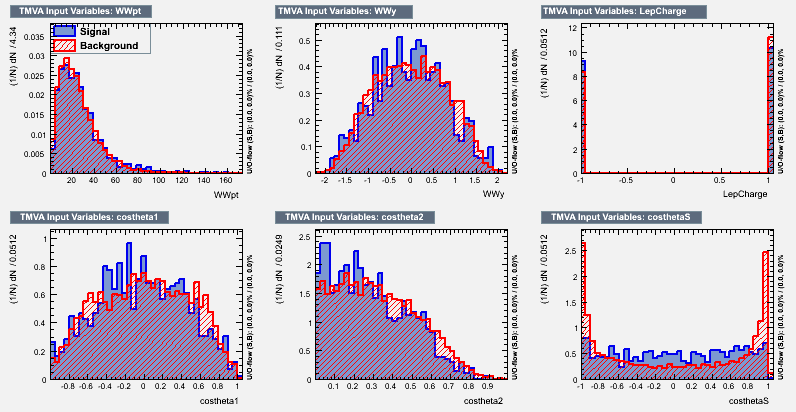
\includegraphics[width=0.8\textwidth]{figs/TMVA_190_nJ2_mu_variables_id_c1.png}
  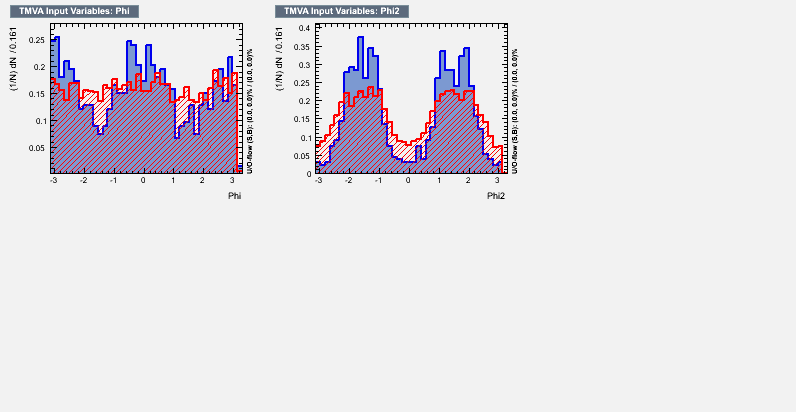
\includegraphics[width=0.8\textwidth]{figs/TMVA_190_nJ2_mu_variables_id_c2.png}	
  \caption{\label{fig:inputs1902jmu}Inputs to the multivariate discriminant for SM Higgs mass of 190~GeV for the 2-jet $W\to\mu\nu$ category}
\end{figure}
%%%%%%%%%%%%%%%%%%%
\newpage
\subsection{Input variables: \texorpdfstring{$M_H$}{M(H)} = 190~GeV, 3 jets}
%%%%%%%%%%%%%%%%%%%
\begin{figure}[ht]
  \centering
  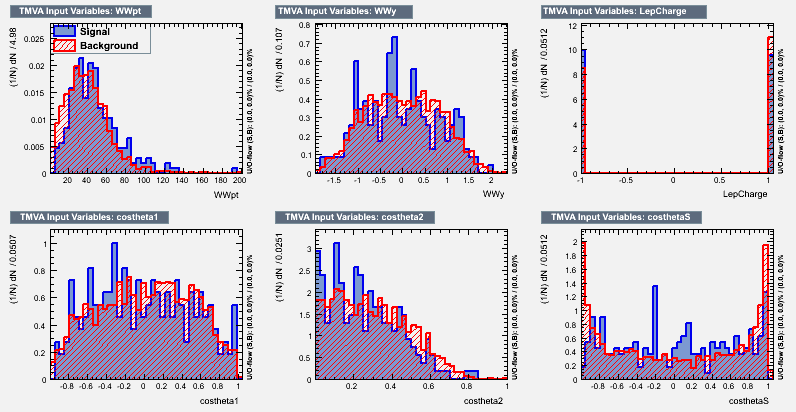
\includegraphics[width=0.8\textwidth]{figs/TMVA_190_nJ3_mu_variables_id_c1.png}
  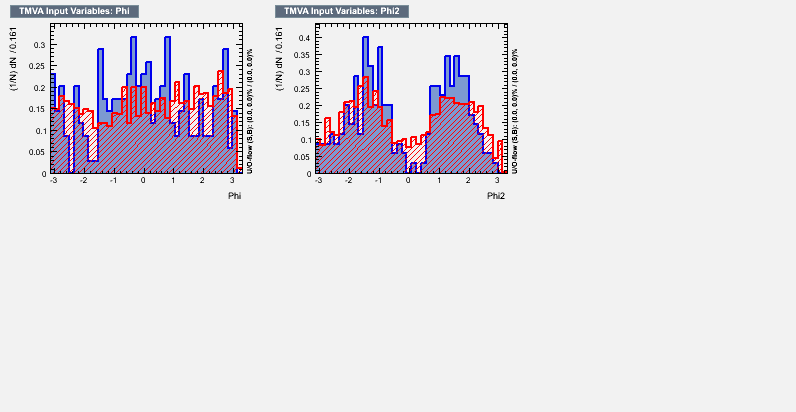
\includegraphics[width=0.8\textwidth]{figs/TMVA_190_nJ3_mu_variables_id_c2.png}	
  \caption{\label{fig:inputs1903jmu}Inputs to the multivariate discriminant for SM Higgs mass of 190~GeV for the 3-jet $W\to\mu\nu$ category}
\end{figure}
%%%%%%%%%%%%%%%%%%%
\newpage
\subsection{Input variables: \texorpdfstring{$M_H$}{M(H)} = 200~GeV, 2 jets}
%%%%%%%%%%%%%%%%%%%
\begin{figure}[ht]
  \centering
  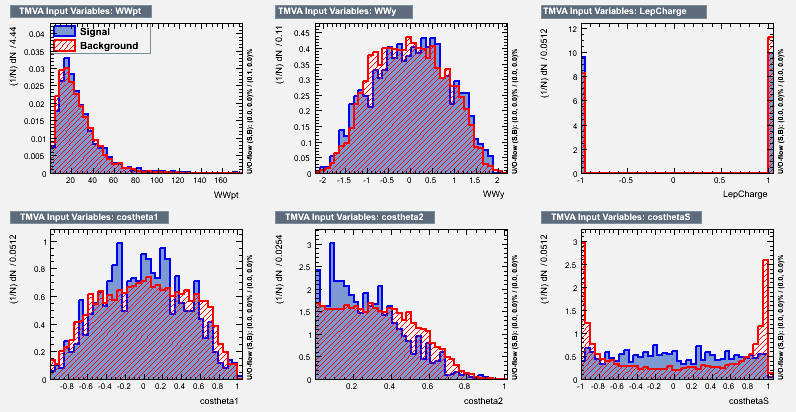
\includegraphics[width=0.8\textwidth]{figs/TMVA_200_nJ2_mu_variables_id_c1.png}
  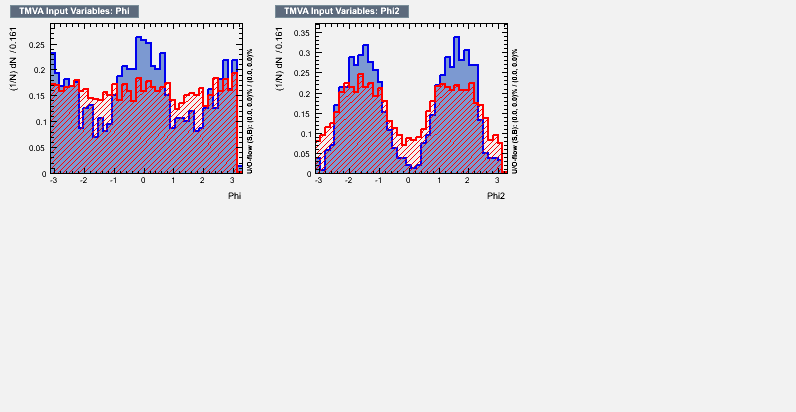
\includegraphics[width=0.8\textwidth]{figs/TMVA_200_nJ2_mu_variables_id_c2.png}	
  \caption{\label{fig:inputs2002jmu}Inputs to the multivariate discriminant for SM Higgs mass of 200~GeV for the 2-jet $W\to\mu\nu$ category}
\end{figure}
%%%%%%%%%%%%%%%%%%%
\newpage
\subsection{Input variables: \texorpdfstring{$M_H$}{M(H)} = 200~GeV, 3 jets}
%%%%%%%%%%%%%%%%%%%
\begin{figure}[ht]
  \centering
  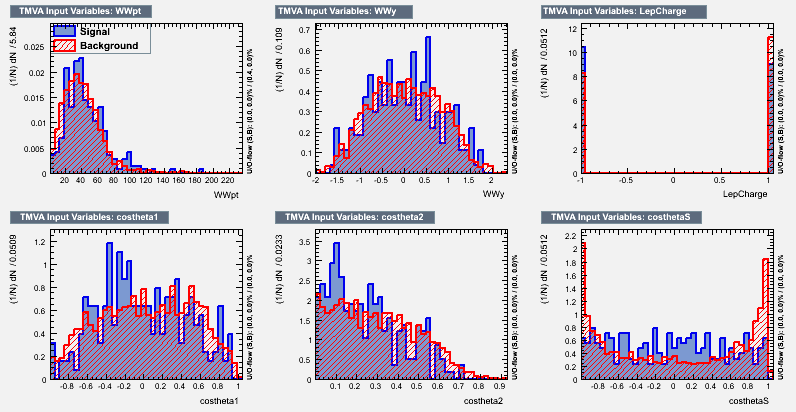
\includegraphics[width=0.8\textwidth]{figs/TMVA_200_nJ3_mu_variables_id_c1.png}
  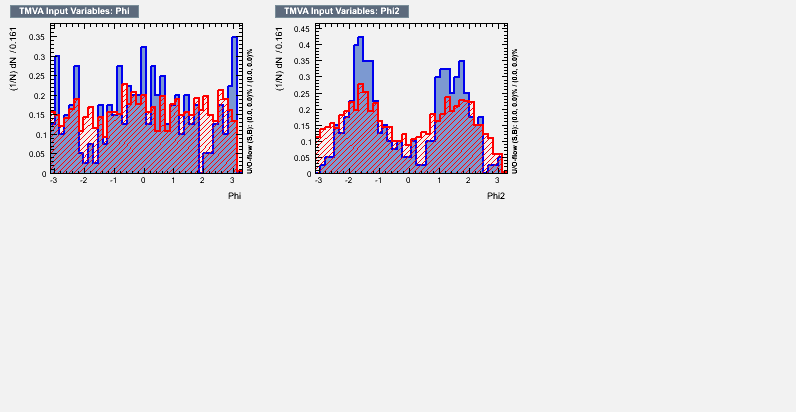
\includegraphics[width=0.8\textwidth]{figs/TMVA_200_nJ3_mu_variables_id_c2.png}	
  \caption{\label{fig:inputs2003jmu}Inputs to the multivariate discriminant for SM Higgs mass of 200~GeV for the 3-jet $W\to\mu\nu$ category}
\end{figure}
%%%%%%%%%%%%%%%%%%%
\newpage
\subsection{Input variables: \texorpdfstring{$M_H$}{M(H)} = 250~GeV, 2 jets}
%%%%%%%%%%%%%%%%%%%
\begin{figure}[ht]
  \centering
  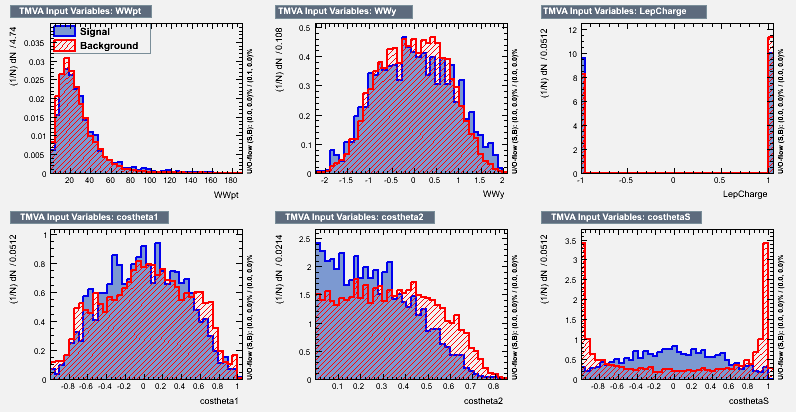
\includegraphics[width=0.8\textwidth]{figs/TMVA_250_nJ2_mu_variables_id_c1.png}
  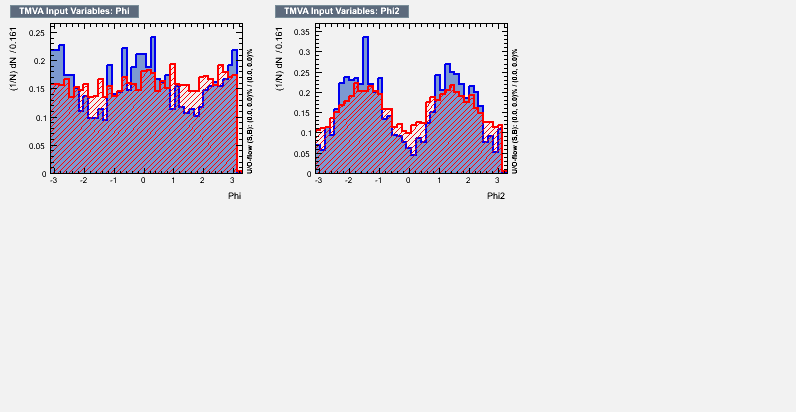
\includegraphics[width=0.8\textwidth]{figs/TMVA_250_nJ2_mu_variables_id_c2.png}	
  \caption{\label{fig:inputs2502jmu}Inputs to the multivariate discriminant for SM Higgs mass of 250~GeV for the 2-jet $W\to\mu\nu$ category}
\end{figure}
%%%%%%%%%%%%%%%%%%%
\newpage
\subsection{Input variables: \texorpdfstring{$M_H$}{M(H)} = 250~GeV, 3 jets}
%%%%%%%%%%%%%%%%%%%
\begin{figure}[ht]
  \centering
  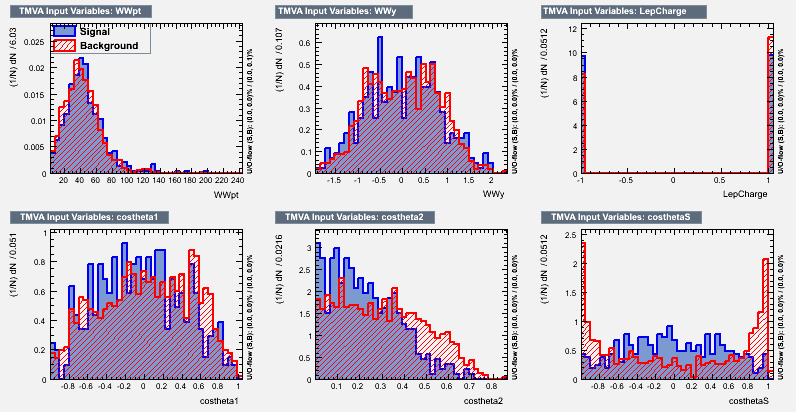
\includegraphics[width=0.8\textwidth]{figs/TMVA_250_nJ3_mu_variables_id_c1.png}
  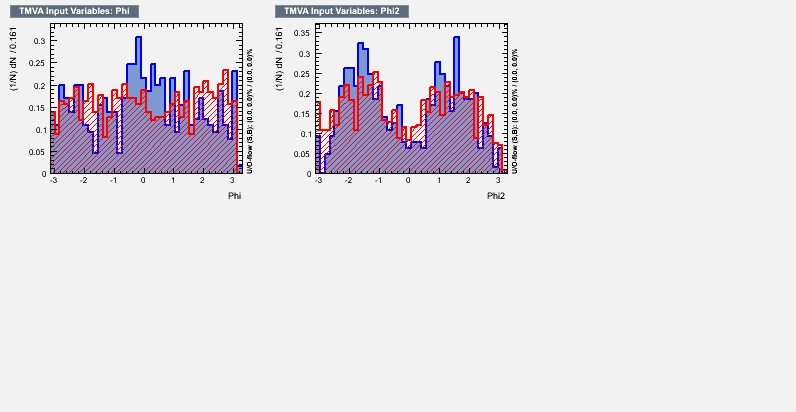
\includegraphics[width=0.8\textwidth]{figs/TMVA_250_nJ3_mu_variables_id_c2.png}	
  \caption{\label{fig:inputs2503jmu}Inputs to the multivariate discriminant for SM Higgs mass of 250~GeV for the 3-jet $W\to\mu\nu$ category}
\end{figure}
%%%%%%%%%%%%%%%%%%%
\newpage
\subsection{Input variables: \texorpdfstring{$M_H$}{M(H)} = 300~GeV, 2 jets}
%%%%%%%%%%%%%%%%%%%
\begin{figure}[ht]
  \centering
  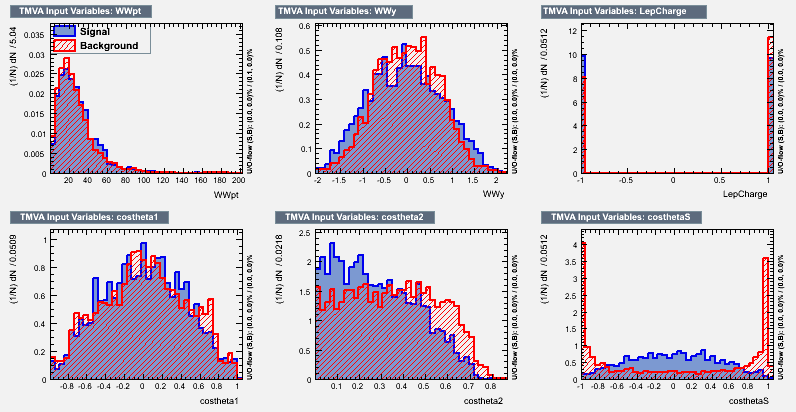
\includegraphics[width=0.8\textwidth]{figs/TMVA_300_nJ2_mu_variables_id_c1.png}
  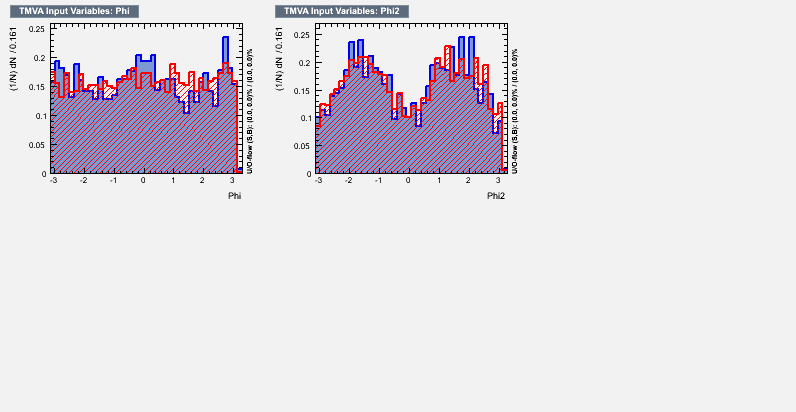
\includegraphics[width=0.8\textwidth]{figs/TMVA_300_nJ2_mu_variables_id_c2.png}	
  \caption{\label{fig:inputs3002jmu}Inputs to the multivariate discriminant for SM Higgs mass of 300~GeV for the 2-jet $W\to\mu\nu$ category}
\end{figure}
%%%%%%%%%%%%%%%%%%%
\newpage
\subsection{Input variables: \texorpdfstring{$M_H$}{M(H)} = 300~GeV, 3 jets}
%%%%%%%%%%%%%%%%%%%
\begin{figure}[ht]
  \centering
  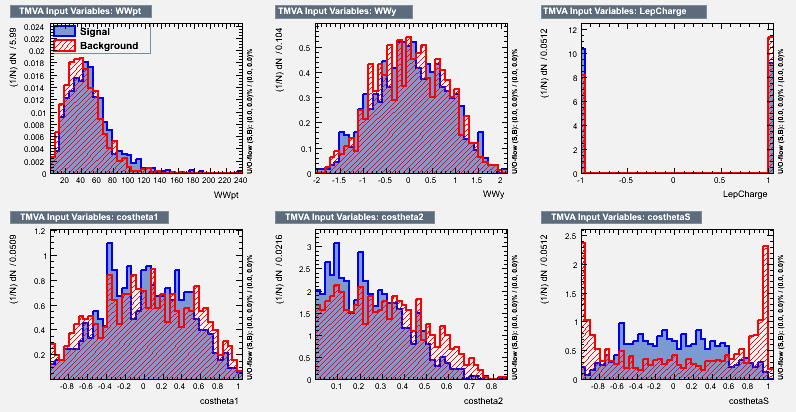
\includegraphics[width=0.8\textwidth]{figs/TMVA_300_nJ3_mu_variables_id_c1.png}
  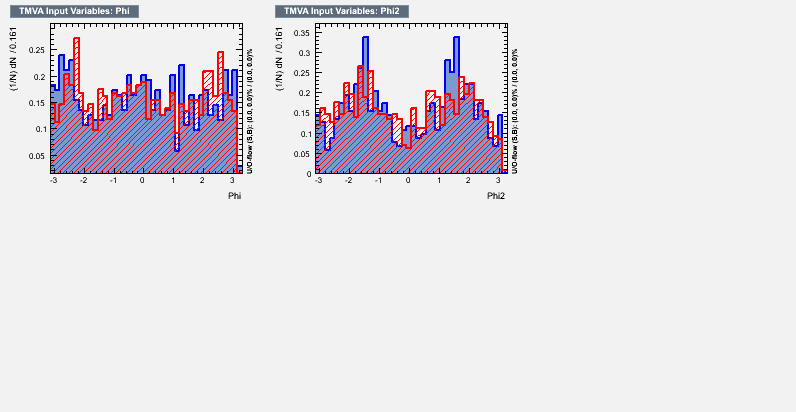
\includegraphics[width=0.8\textwidth]{figs/TMVA_300_nJ3_mu_variables_id_c2.png}	
  \caption{\label{fig:inputs3003jmu}Inputs to the multivariate discriminant for SM Higgs mass of 300~GeV for the 3-jet $W\to\mu\nu$ category}
\end{figure}
%%%%%%%%%%%%%%%%%%%
\newpage
\subsection{Input variables: \texorpdfstring{$M_H$}{M(H)} = 350~GeV, 2 jets}
%%%%%%%%%%%%%%%%%%%
\begin{figure}[ht]
  \centering
  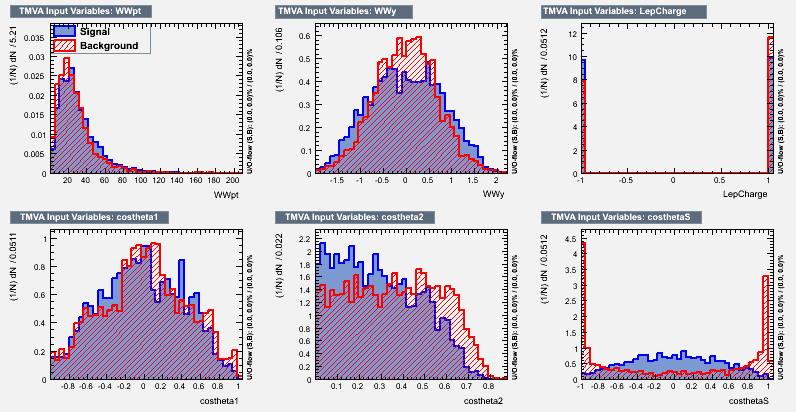
\includegraphics[width=0.8\textwidth]{figs/TMVA_350_nJ2_mu_variables_id_c1.png}
  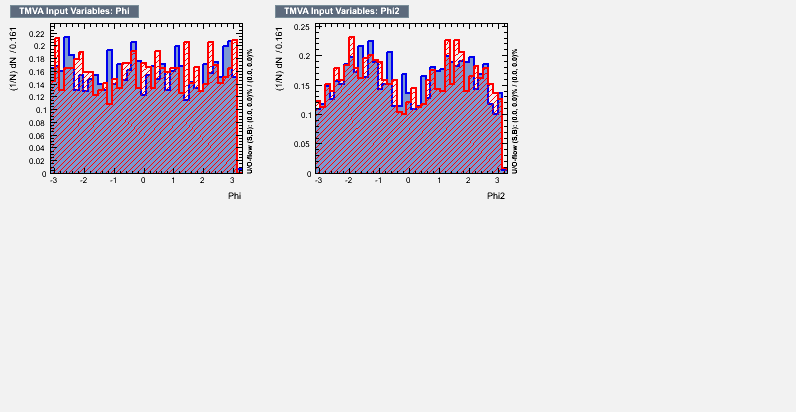
\includegraphics[width=0.8\textwidth]{figs/TMVA_350_nJ2_mu_variables_id_c2.png}	
  \caption{\label{fig:inputs3502jmu}Inputs to the multivariate discriminant for SM Higgs mass of 350~GeV for the 2-jet $W\to\mu\nu$ category}
\end{figure}
%%%%%%%%%%%%%%%%%%%
\newpage
\subsection{Input variables: \texorpdfstring{$M_H$}{M(H)} = 350~GeV, 3 jets}
%%%%%%%%%%%%%%%%%%%
\begin{figure}[ht]
  \centering
  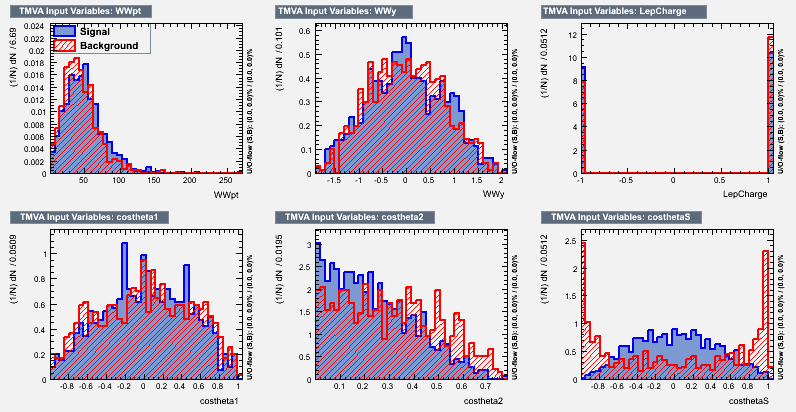
\includegraphics[width=0.8\textwidth]{figs/TMVA_350_nJ3_mu_variables_id_c1.png}
  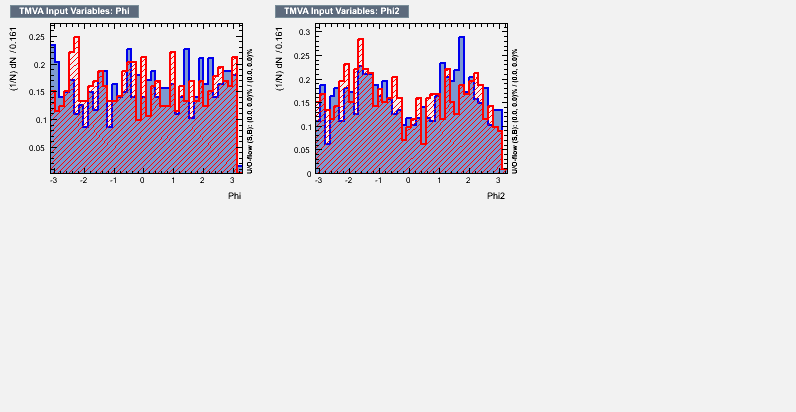
\includegraphics[width=0.8\textwidth]{figs/TMVA_350_nJ3_mu_variables_id_c2.png}	
  \caption{\label{fig:inputs3503jmu}Inputs to the multivariate discriminant for SM Higgs mass of 350~GeV for the 3-jet $W\to\mu\nu$ category}
\end{figure}
%%%%%%%%%%%%%%%%%%%
\newpage
\subsection{Input variables: \texorpdfstring{$M_H$}{M(H)} = 400~GeV, 2 jets}
%%%%%%%%%%%%%%%%%%%
\begin{figure}[ht]
  \centering
  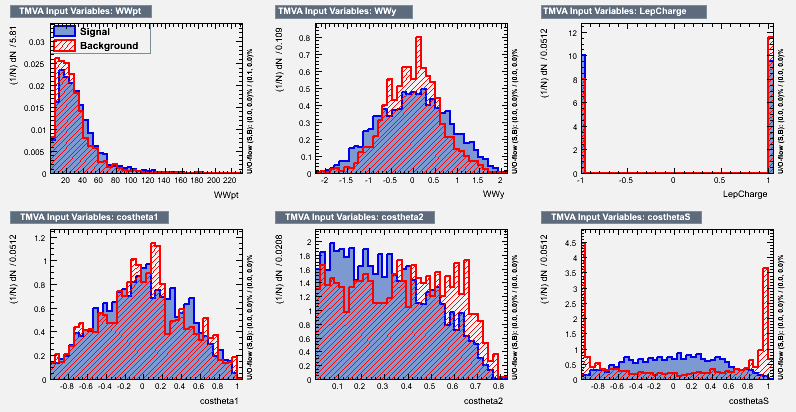
\includegraphics[width=0.8\textwidth]{figs/TMVA_400_nJ2_mu_variables_id_c1.png}
  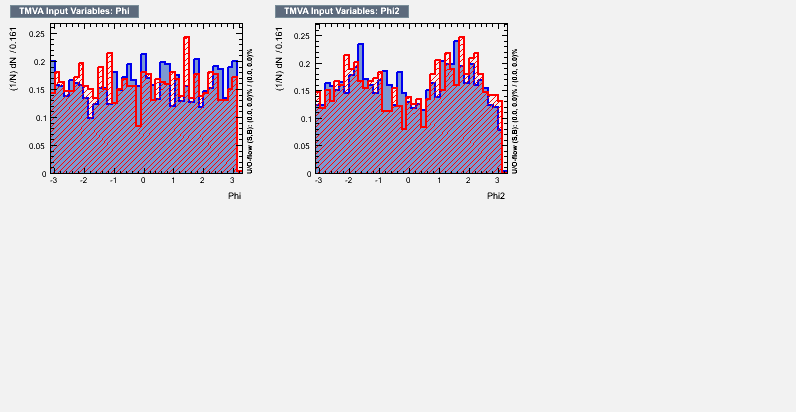
\includegraphics[width=0.8\textwidth]{figs/TMVA_400_nJ2_mu_variables_id_c2.png}	
  \caption{\label{fig:inputs4002jmu}Inputs to the multivariate discriminant for SM Higgs mass of 400~GeV for the 2-jet $W\to\mu\nu$ category}
\end{figure}
%%%%%%%%%%%%%%%%%%%
\newpage
\subsection{Input variables: \texorpdfstring{$M_H$}{M(H)} = 400~GeV, 3 jets}
%%%%%%%%%%%%%%%%%%%
\begin{figure}[ht]
  \centering
  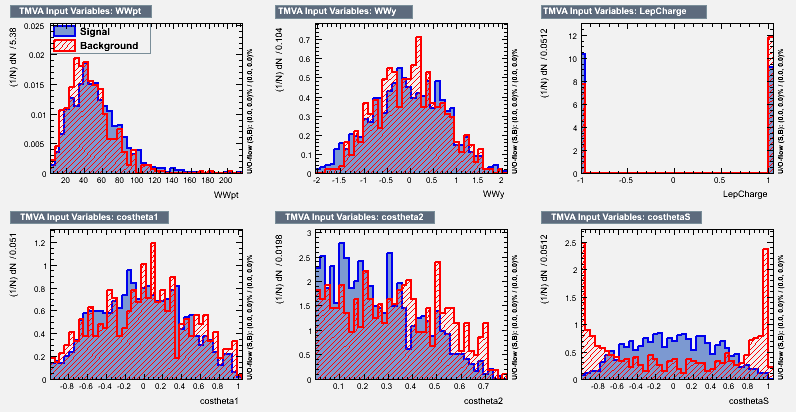
\includegraphics[width=0.8\textwidth]{figs/TMVA_400_nJ3_mu_variables_id_c1.png}
  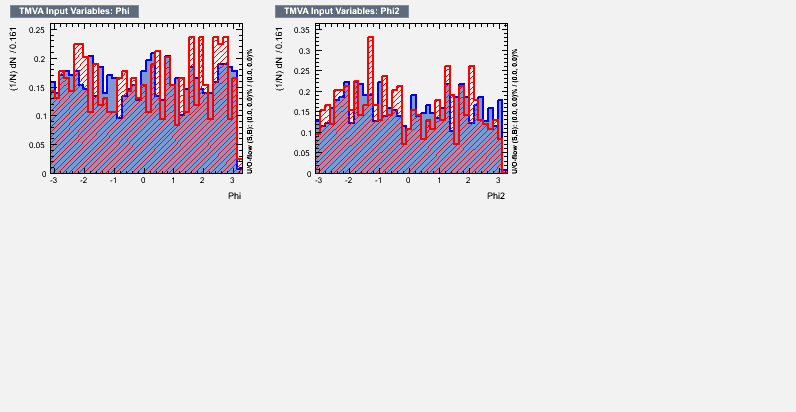
\includegraphics[width=0.8\textwidth]{figs/TMVA_400_nJ3_mu_variables_id_c2.png}	
  \caption{\label{fig:inputs4003jmu}Inputs to the multivariate discriminant for SM Higgs mass of 400~GeV for the 3-jet $W\to\mu\nu$ category}
\end{figure}
%%%%%%%%%%%%%%%%%%%
\newpage
\subsection{Input variables: \texorpdfstring{$M_H$}{M(H)} = 450~GeV, 2 jets}
%%%%%%%%%%%%%%%%%%%
\begin{figure}[ht]
  \centering
  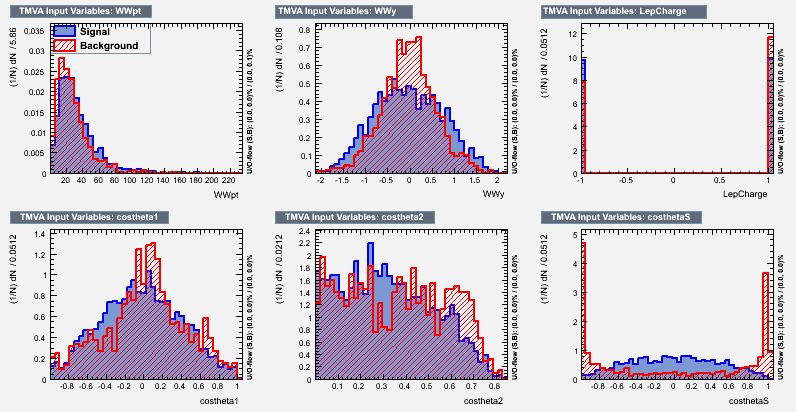
\includegraphics[width=0.8\textwidth]{figs/TMVA_450_nJ2_mu_variables_id_c1.png}
  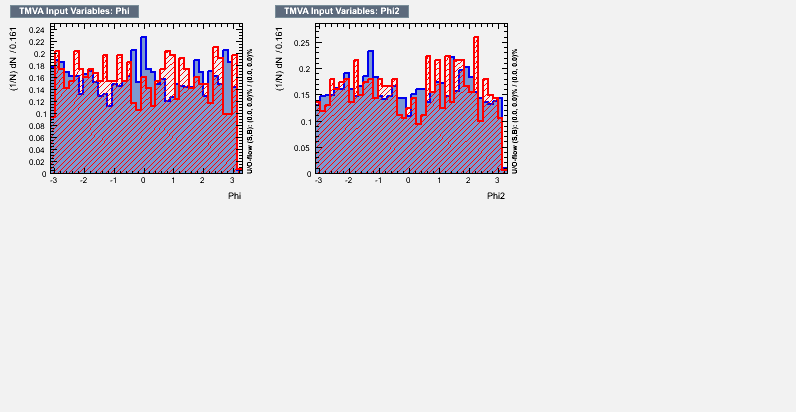
\includegraphics[width=0.8\textwidth]{figs/TMVA_450_nJ2_mu_variables_id_c2.png}	
  \caption{\label{fig:inputs4502jmu}Inputs to the multivariate discriminant for SM Higgs mass of 450~GeV for the 2-jet $W\to\mu\nu$ category}
\end{figure}
%%%%%%%%%%%%%%%%%%%
\newpage
\subsection{Input variables: \texorpdfstring{$M_H$}{M(H)} = 450~GeV, 3 jets}
%%%%%%%%%%%%%%%%%%%
\begin{figure}[ht]
  \centering
  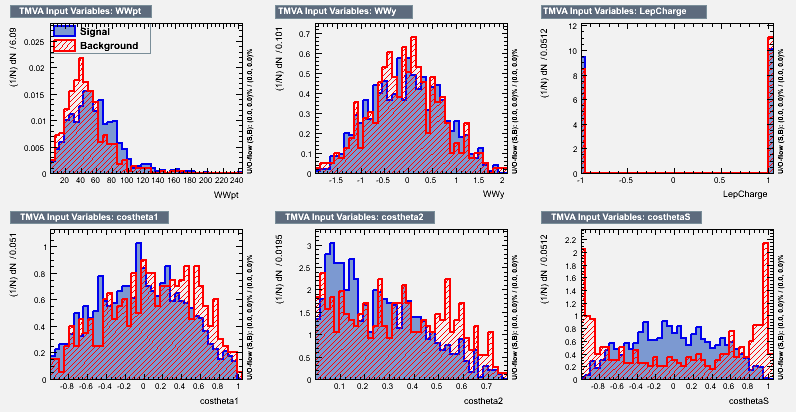
\includegraphics[width=0.8\textwidth]{figs/TMVA_450_nJ3_mu_variables_id_c1.png}
  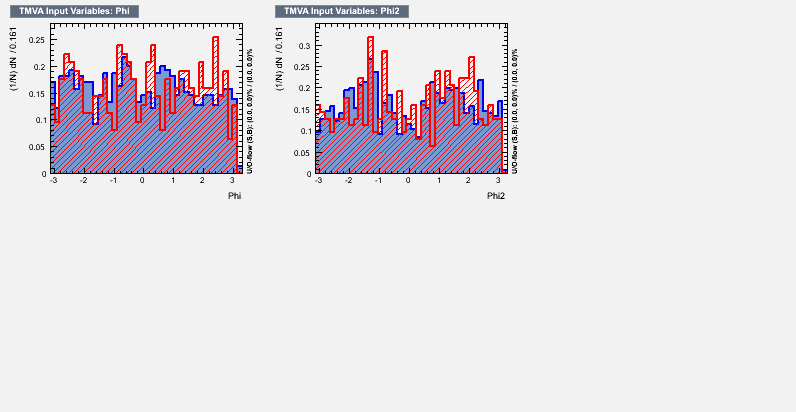
\includegraphics[width=0.8\textwidth]{figs/TMVA_450_nJ3_mu_variables_id_c2.png}	
  \caption{\label{fig:inputs4503jmu}Inputs to the multivariate discriminant for SM Higgs mass of 450~GeV for the 3-jet $W\to\mu\nu$ category}
\end{figure}
%%%%%%%%%%%%%%%%%%%
\newpage
\subsection{Input variables: \texorpdfstring{$M_H$}{M(H)} = 500~GeV, 2 jets}
%%%%%%%%%%%%%%%%%%%
\begin{figure}[ht]
  \centering
  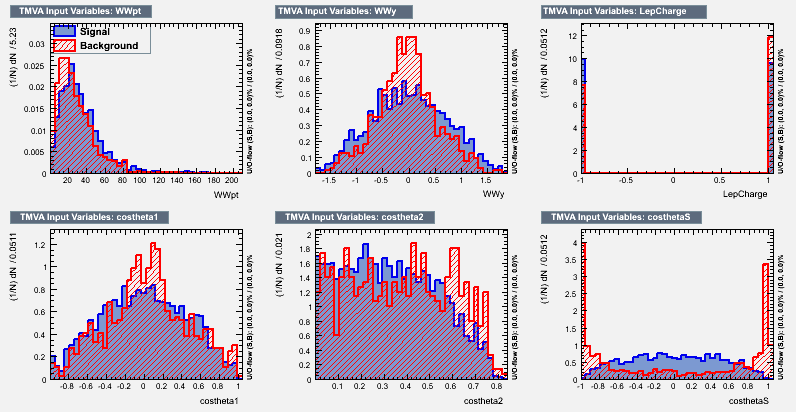
\includegraphics[width=0.8\textwidth]{figs/TMVA_500_nJ2_mu_variables_id_c1.png}
  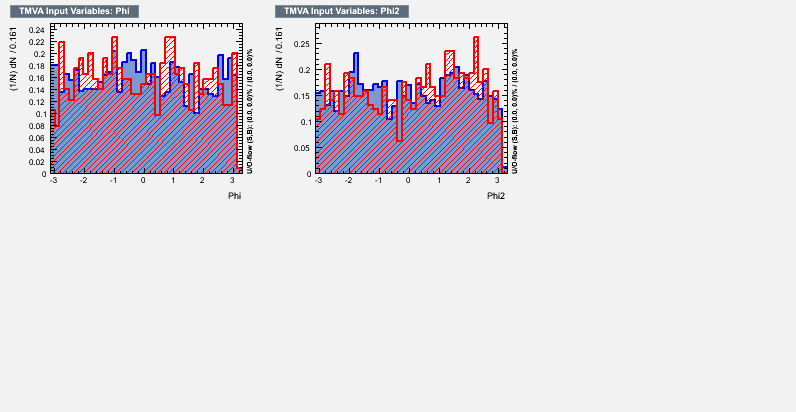
\includegraphics[width=0.8\textwidth]{figs/TMVA_500_nJ2_mu_variables_id_c2.png}	
  \caption{\label{fig:inputs5002jmu}Inputs to the multivariate discriminant for SM Higgs mass of 500~GeV for the 2-jet $W\to\mu\nu$ category}
\end{figure}
%%%%%%%%%%%%%%%%%%%
\newpage
\subsection{Input variables: \texorpdfstring{$M_H$}{M(H)} = 500~GeV, 3 jets}
%%%%%%%%%%%%%%%%%%%
\begin{figure}[ht]
  \centering
  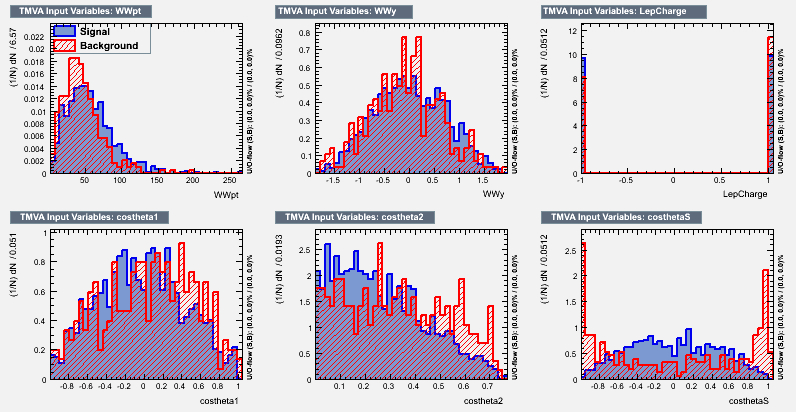
\includegraphics[width=0.8\textwidth]{figs/TMVA_500_nJ3_mu_variables_id_c1.png}
  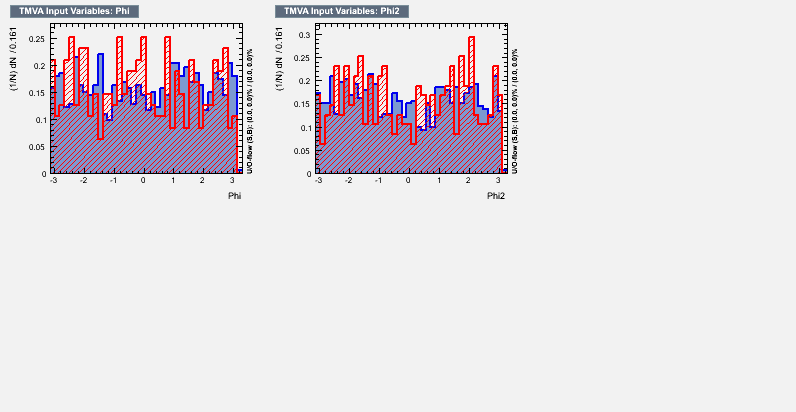
\includegraphics[width=0.8\textwidth]{figs/TMVA_500_nJ3_mu_variables_id_c2.png}	
  \caption{\label{fig:inputs5003jmu}Inputs to the multivariate discriminant for SM Higgs mass of 500~GeV for the 3-jet $W\to\mu\nu$ category}
\end{figure}
%%%%%%%%%%%%%%%%%%%
\newpage
\subsection{Input variables: \texorpdfstring{$M_H$}{M(H)} = 550~GeV, 2 jets}
%%%%%%%%%%%%%%%%%%%
\begin{figure}[ht]
  \centering
  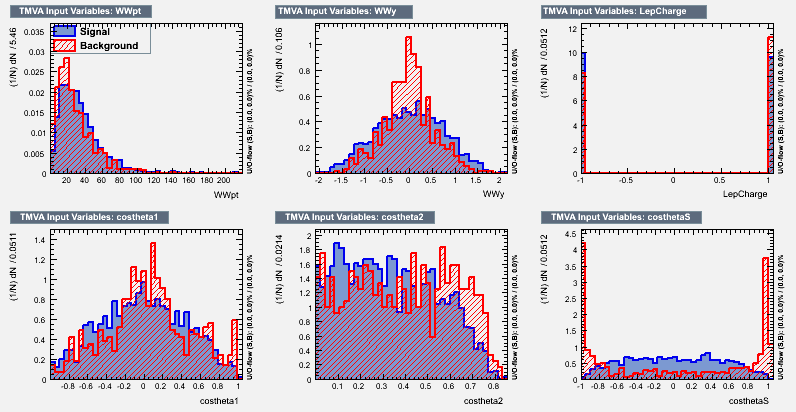
\includegraphics[width=0.8\textwidth]{figs/TMVA_550_nJ2_mu_variables_id_c1.png}
  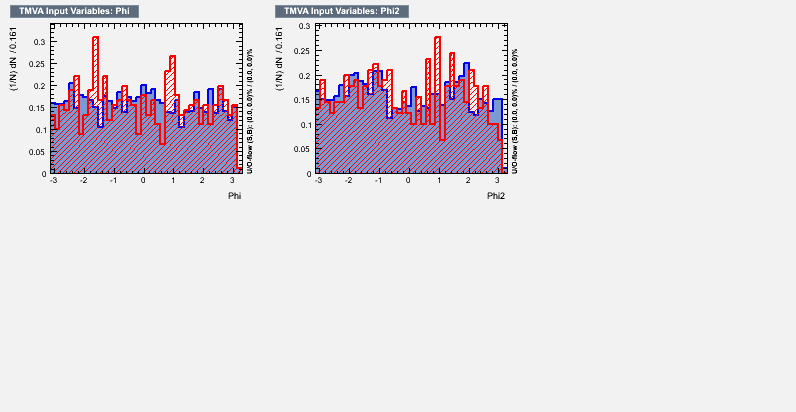
\includegraphics[width=0.8\textwidth]{figs/TMVA_550_nJ2_mu_variables_id_c2.png}	
  \caption{\label{fig:inputs5502jmu}Inputs to the multivariate discriminant for SM Higgs mass of 550~GeV for the 2-jet $W\to\mu\nu$ category}
\end{figure}
%%%%%%%%%%%%%%%%%%%
\newpage
\subsection{Input variables: \texorpdfstring{$M_H$}{M(H)} = 550~GeV, 3 jets}
%%%%%%%%%%%%%%%%%%%
\begin{figure}[ht]
  \centering
  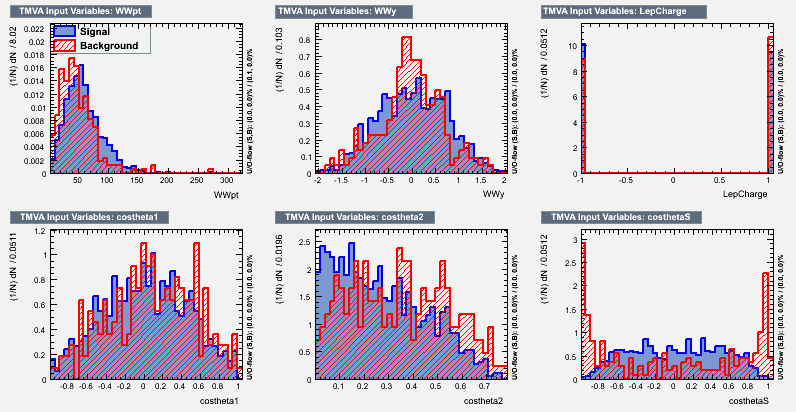
\includegraphics[width=0.8\textwidth]{figs/TMVA_550_nJ3_mu_variables_id_c1.png}
  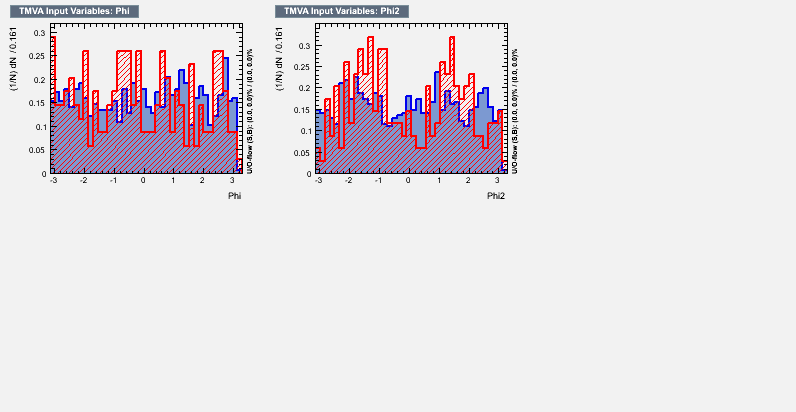
\includegraphics[width=0.8\textwidth]{figs/TMVA_550_nJ3_mu_variables_id_c2.png}	
  \caption{\label{fig:inputs5503jmu}Inputs to the multivariate discriminant for SM Higgs mass of 550~GeV for the 3-jet $W\to\mu\nu$ category}
\end{figure}
%%%%%%%%%%%%%%%%%%%
\newpage
\subsection{Input variables: \texorpdfstring{$M_H$}{M(H)} = 600~GeV, 2 jets}
%%%%%%%%%%%%%%%%%%%
\begin{figure}[ht]
  \centering
  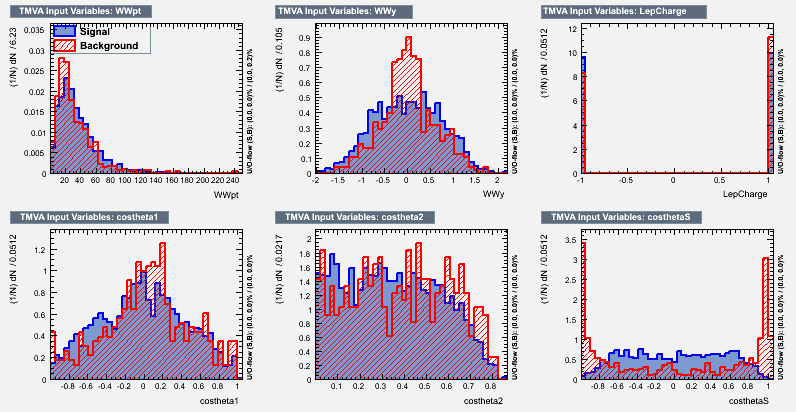
\includegraphics[width=0.8\textwidth]{figs/TMVA_600_nJ2_mu_variables_id_c1.png}
  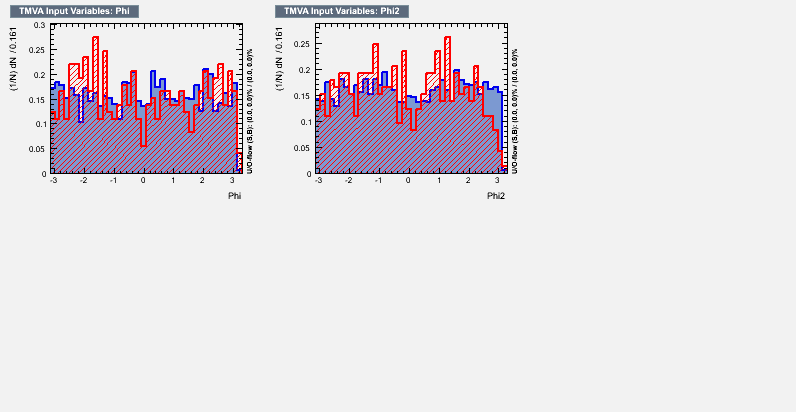
\includegraphics[width=0.8\textwidth]{figs/TMVA_600_nJ2_mu_variables_id_c2.png}	
  \caption{\label{fig:inputs6002jmu}Inputs to the multivariate discriminant for SM Higgs mass of 600~GeV for the 2-jet $W\to\mu\nu$ category}
\end{figure}
%%%%%%%%%%%%%%%%%%%
\newpage
\subsection{Input variables: \texorpdfstring{$M_H$}{M(H)} = 600~GeV, 3 jets}
%%%%%%%%%%%%%%%%%%%
\begin{figure}[ht]
  \centering
  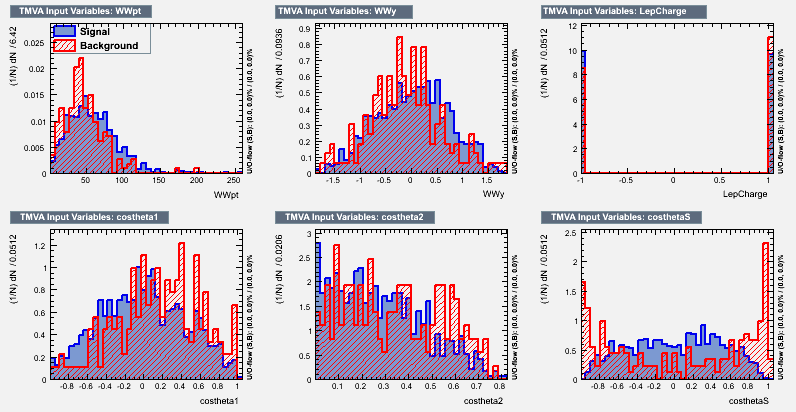
\includegraphics[width=0.8\textwidth]{figs/TMVA_600_nJ3_mu_variables_id_c1.png}
  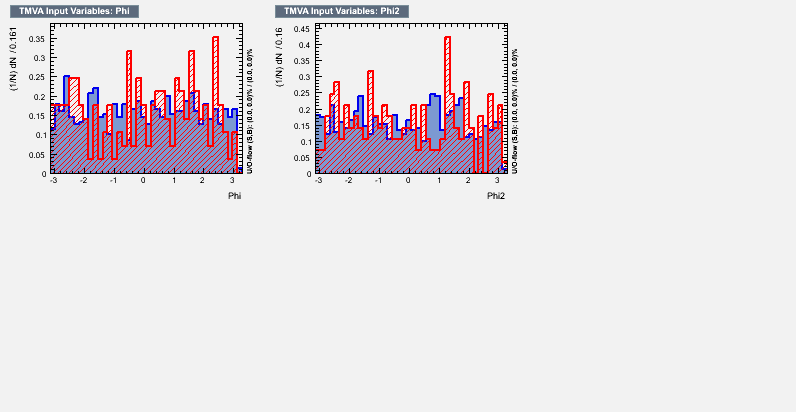
\includegraphics[width=0.8\textwidth]{figs/TMVA_600_nJ3_mu_variables_id_c2.png}	
  \caption{\label{fig:inputs6003jmu}Inputs to the multivariate discriminant for SM Higgs mass of 600~GeV for the 3-jet $W\to\mu\nu$ category}
\end{figure}
%%%%%%%%%%%%%%%%%%%
